\chapter{Software}

\section{Introducci\'on}

Para poder llevar a cabo el objetivo de este informe se pretende primero reproducir los resultados del art\'iculo de Carnicero (2013). Esto con el fin de probar los programas generados por el estudiante del doctorado y as\'i, posteriormente aplicarlos en el objetivo de este trabajo de investigaci\'on. Procediendo de esta manera, se descargaron de internet (\href{http://infomet.am.ub.es/clima/gijon/}{\emph{http://infomet.am.ub.es/clima/gijon/}}) los datos circulares-lineales del art\'iculo de Carnicero los cuales corresponden a datos de direcci\'on del viento y precipitaci\'on del 06/Noviembre/1994--31/Enero/2009 de una estaci\'on meteorol\'ogica en Somi\'o (Espa\~na). Posteriormente, para verificar la validez de los datos se realiz\'o el mismo an\'alisis exploratorio que se muestra en el art\'iculo con el fin de confirmar que los datos son los mismos. Las direcciones del viento est\'an dadas en grados (0$^\circ$-359$^\circ$).

\section{Validaci\'on del software}
A continuaci\'on se muestran los gr\'aficos an\'alogos a los presentados en dicho art\'iculo.

\begin{figure}
	\centering
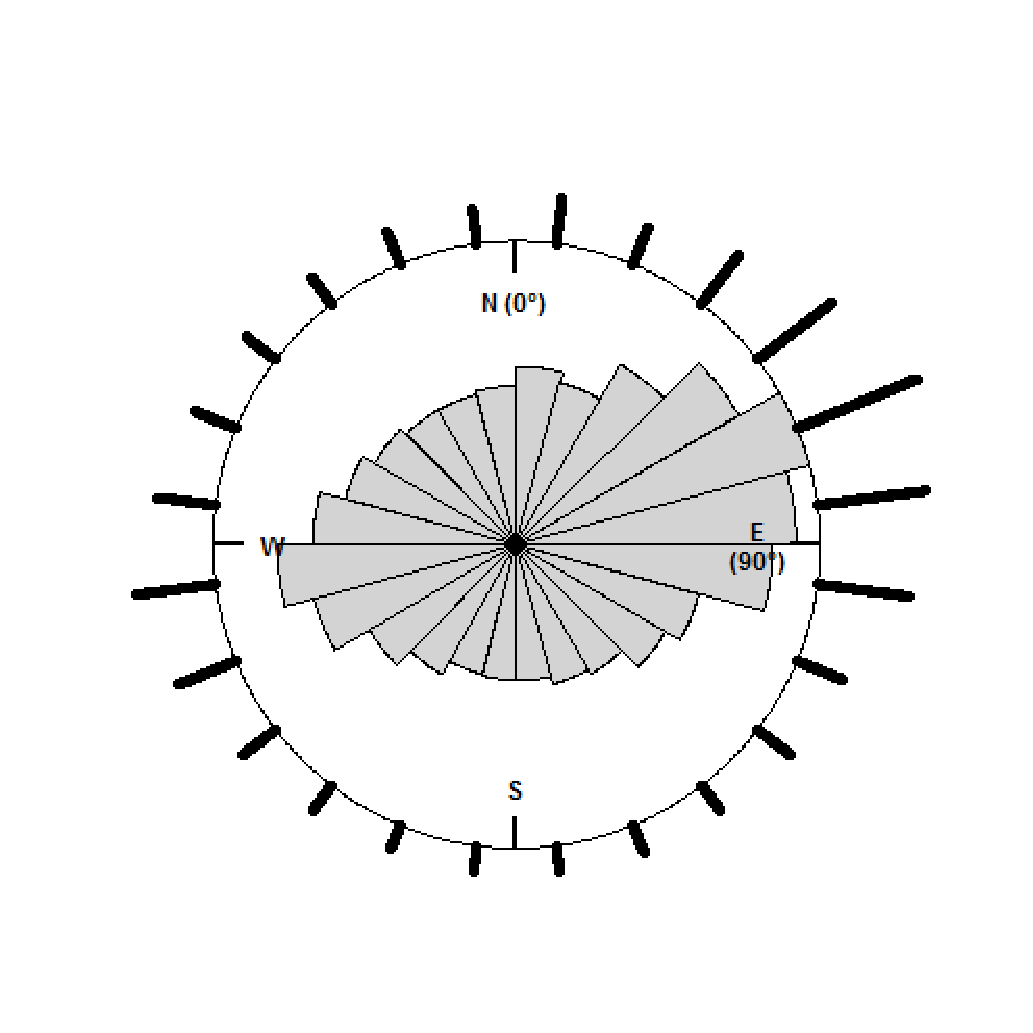
\includegraphics[width=2.75197in,height=2.75197in]{image1} 
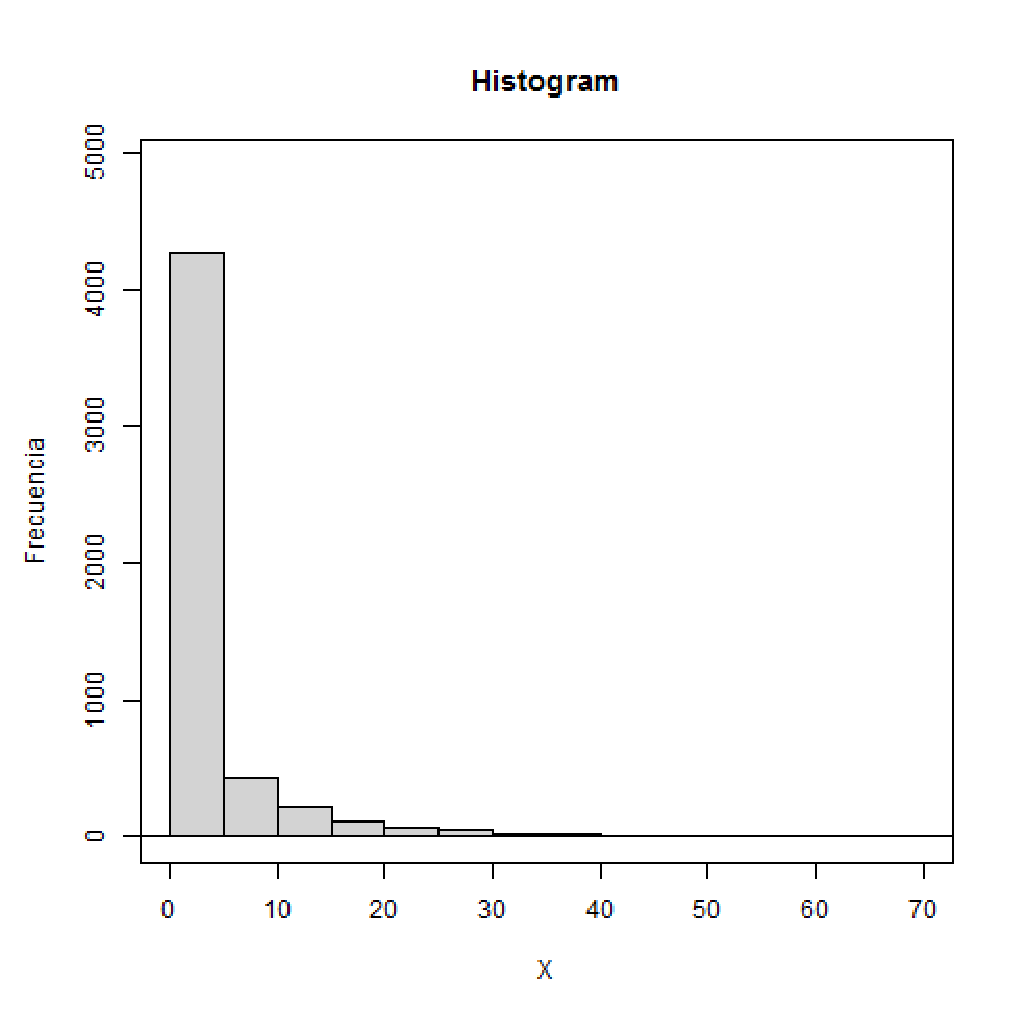
\includegraphics[width=2.75197in,height=2.75197in]{image3} 
	\caption{(izquierda) Roseta de orientaciones, (derecha) histograma de precipitaci\'on.}
	\label{f:gijonEDA1D}
\end{figure}

\begin{figure}
	\centering
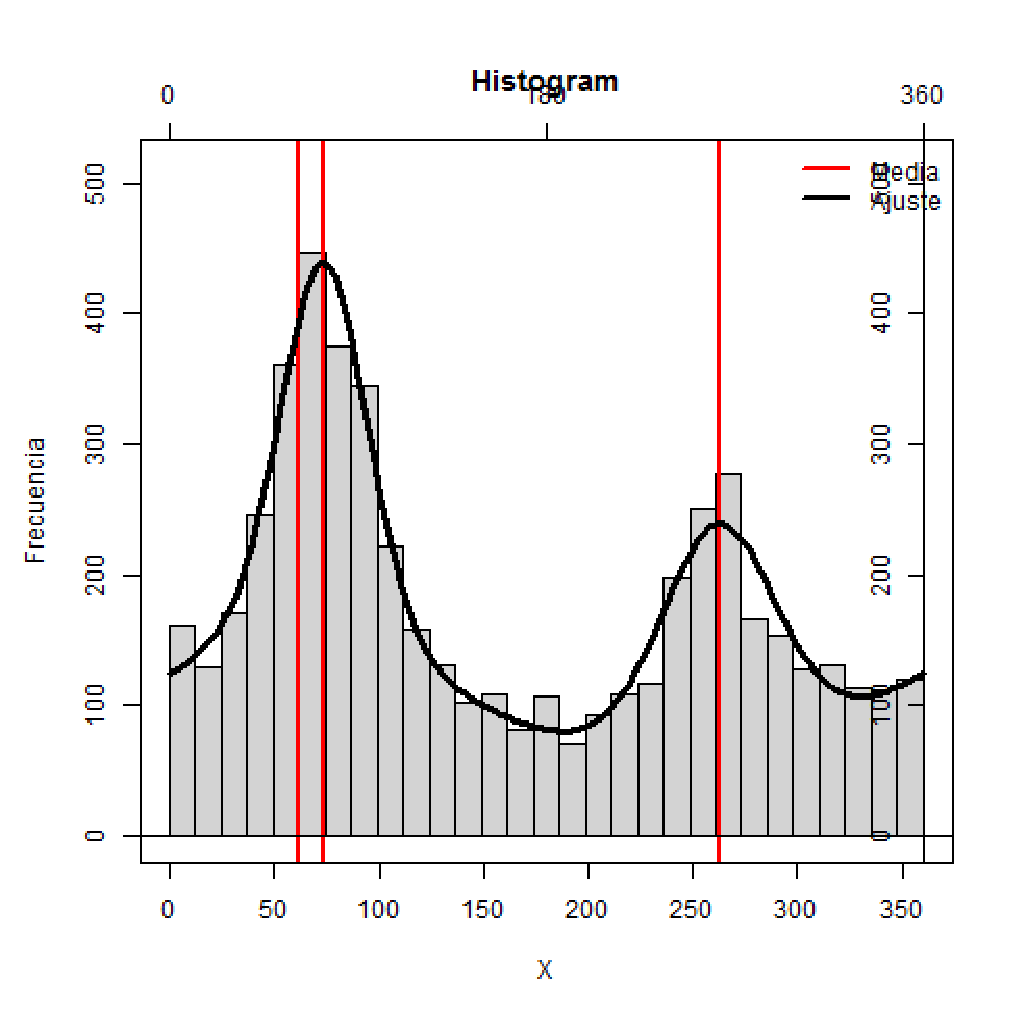
\includegraphics[width=2.75197in,height=2.75197in]{image5} 
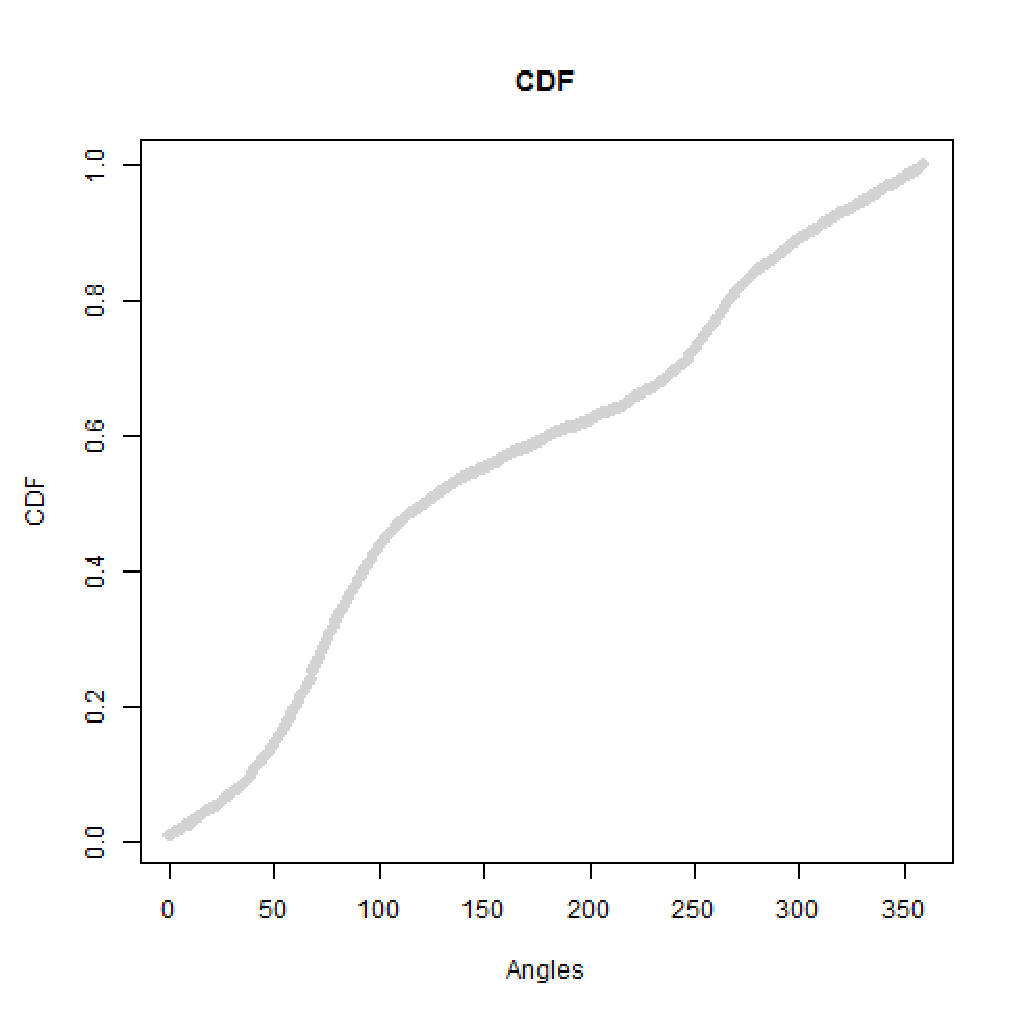
\includegraphics[width=2.75197in,height=2.75197in]{image7} 
	\caption{Figuras equivalentes a la Fig. 2 del art\'iculo.(recuadros superiores) Densidad marginal estimada, (recuadros inferiores) funciones de distribuci\'on acumulada, para la direcci\'on del viento (izquierda) y para la precipitaci\'on pluvial (derecha)}
	\label{f:gijonModels1D}
\end{figure}

\begin{figure}
	\centering
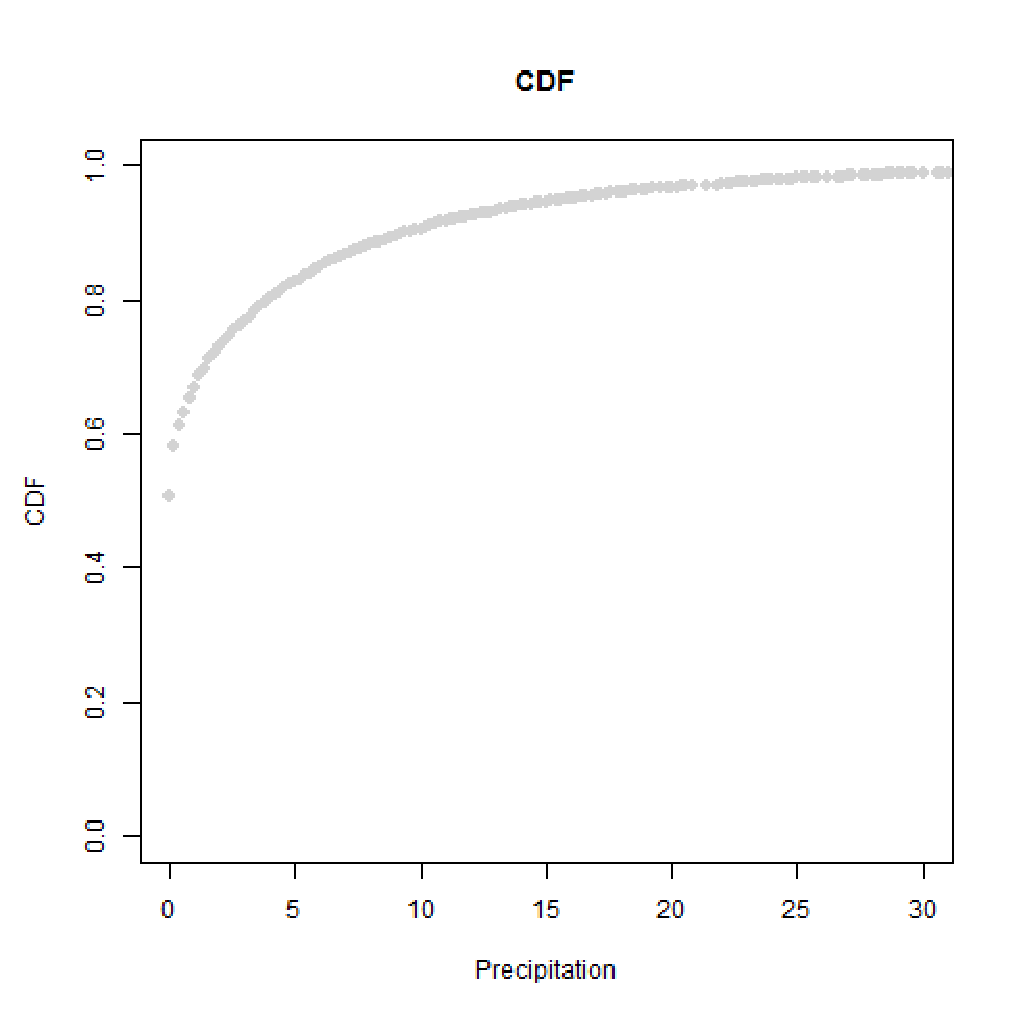
\includegraphics[width=2.75197in,height=2.75197in]{image9} 
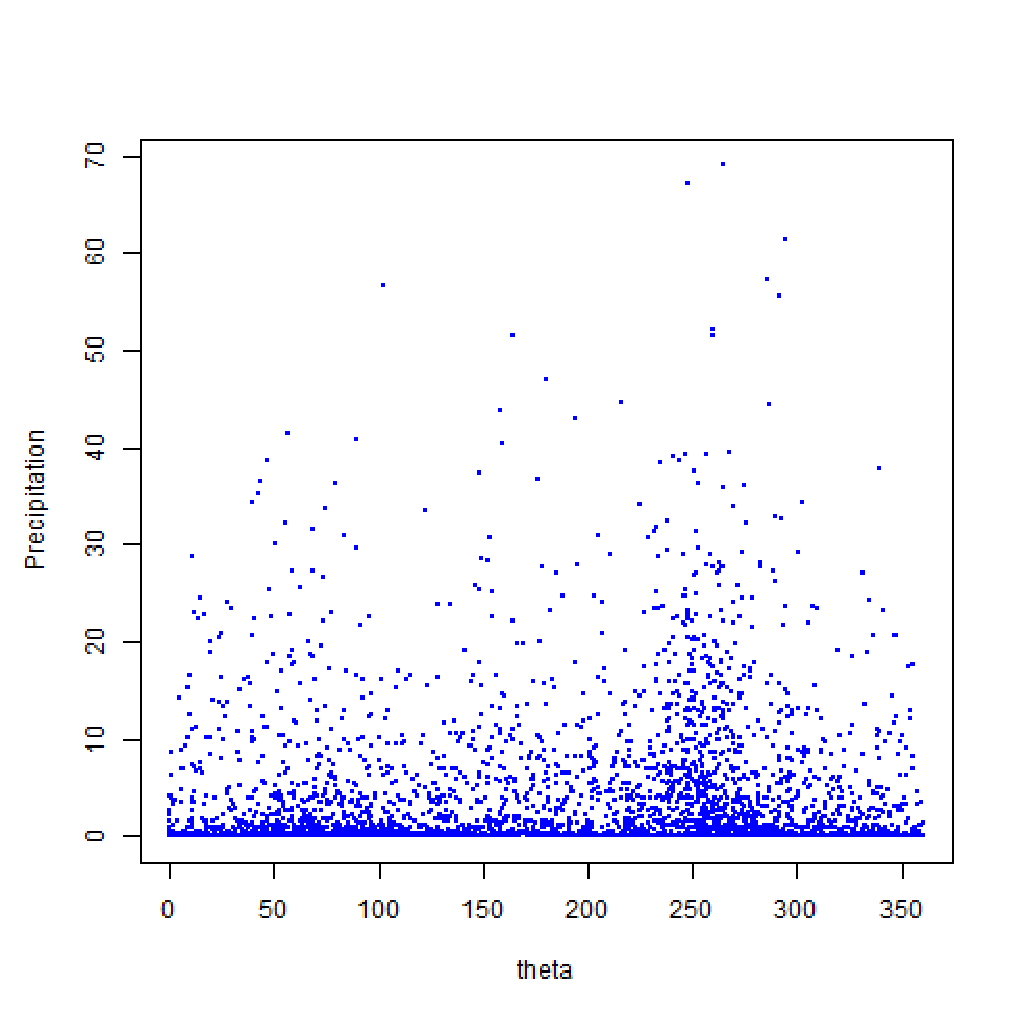
\includegraphics[width=2.75000in,height=2.75000in]{image11}
	\caption{Figura equivalentes a la Fig. 4 del art\'iculo. Diagrama de dispersi\'on de precipitaci\'on y direcci\'on del viento (theta).}
	\label{f:gijonDens2D}
\end{figure}

A continuaci\'on se procede a implementar los modelos matem\'aticos (Carnicero, 2013) de c\'opulas no param\'etricas para datos circulares-lineales. Estos modelos fueron implementados en el paquete estad\'istico R.

La densidad de c\'opula obtenida se muestra en la siguiente figura:

\begin{figure}
	\centering
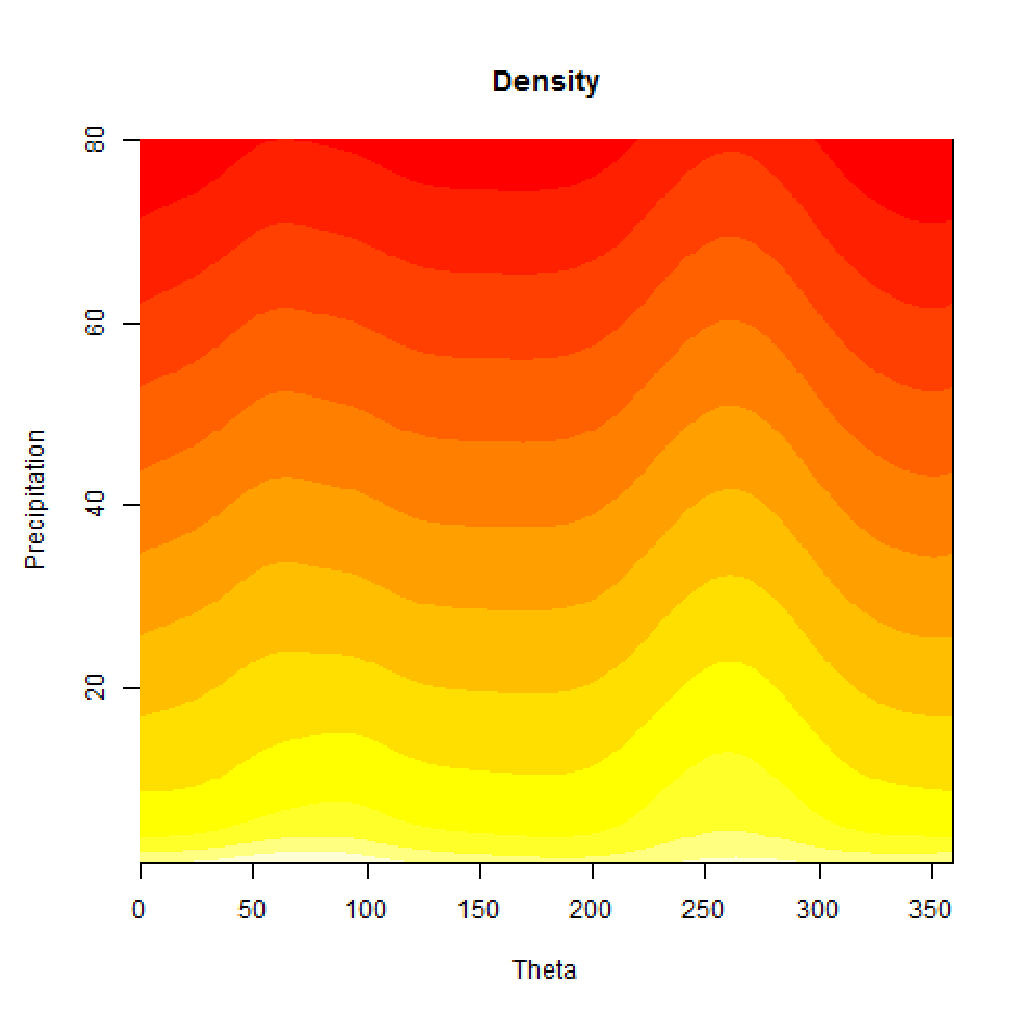
\includegraphics[width=3.50000in,height=3.50000in]{image13}
	\caption{Densidad de c\'opula.}
	\label{f:gijonDens2Dpixels}
\end{figure}

Una vez reproducidos los datos del trabajo de Carnicero, se sabe que los programas computacionales funcionan correctamente. El siguiente paso ser\'ia implementar la simulaci\'on de dicho modelo de c\'opula.

Dado un modelo de dependencia (c\'opula), uno de los objetivos perseguidos al modelar la funci\'on de densidad de probabilidad conjunta es simular valores de las variables aleatorias, lo cual se llevar\'a a cabo utilizando la metodolog\'ia (Erdely-Ruiz \& D\'iaz-Viera, 2012) de la secci\'on denominada \emph{Simulaci\'on conjunta de variables aleatorias} de la \emph{Unidad Te\'orica B}. Atendiendo al punto 1 de dicha metodolog\'ia es necesario simular valores con una distribuci\'on uniforme en el intervalo \(\left\lbrack 0,1 \right\rbrack\), ya que estos son requeridos por la c\'opula. Esto se puede conseguir con la funci\'on \emph{runif} del paquete \emph{base}. Recu\'erdese que la c\'opula bivariada tiene dominio \(\left\lbrack 0,1 \right\rbrack^{2}\). Para el segundo paso se requieren a) la C\'opula; b) obtener una funci\'on inversa. Al terminar este segundo paso se cuenta con dos conjuntos de valores \(\left\{ u_{i} \right\}\) y \(\left\{ v_{i} \right\}\) que est\'an distribuidos uniformemente pero que conservan la misma dependencia que los datos originales. Por \'ultimo, para el tercer paso, los datos simulados, \(\left\{ \left( x_{i},y_{i} \right) \right\}\), se obtienen utilizando funciones cuantiles no param\'etricas de \(X\) y \(Y\) respectivamente. Estos funciones \(\tilde{Q}\) y \(\tilde{R}\) son estimadas mediante polinomios de Bernstein-Kantorovich \citep{munoz-perez_estimating_1987}. La Figura 2 muestra un ejemplo de un conjunto de datos a los cuales se les model\'o su funci\'on de distribuci\'on con los polinomios de Bernstein-Kantorovich. Por lo tanto \(\left( x_{i},y_{i} \right) = \left( \tilde{Q}\left( u_{i} \right),\tilde{R}\left( v_{i} \right) \right)\).
La implementaci\'on computacional de estas funciones cuantiles se encuentra en el paquete \verb|lmomco| bajo el nombre de \verb|dat2bernqua|.

\begin{figure}
	\centering
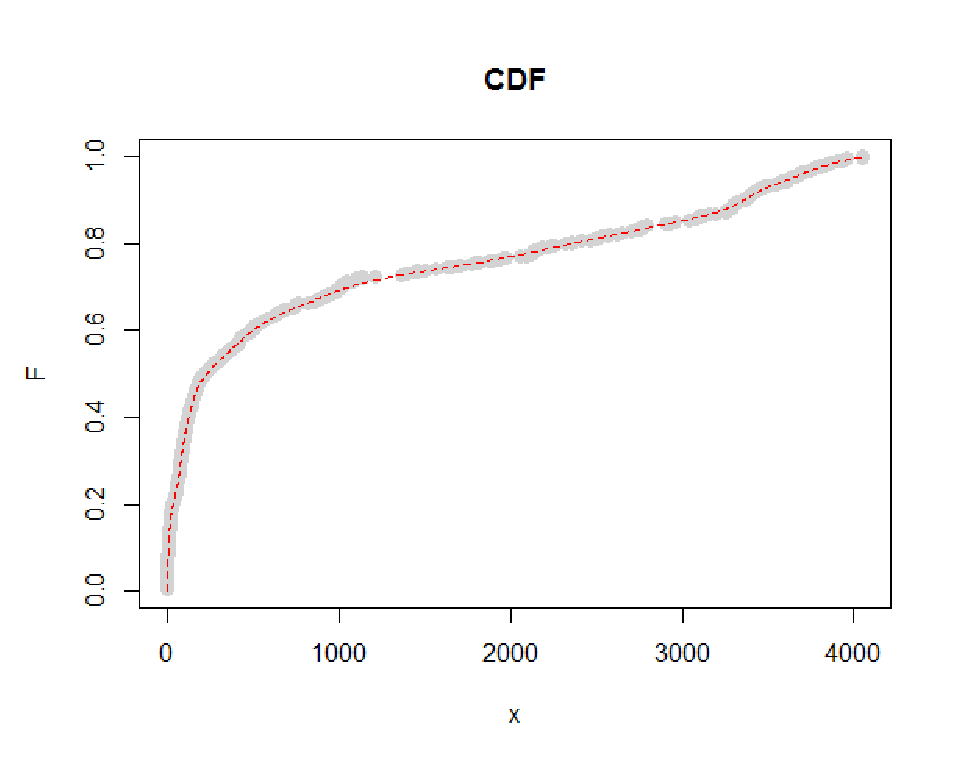
\includegraphics[width=3.83512in,height=3.04275in]{image14}
	\caption{Funci\'on de densidad de probabilidad emp\'irica y ajustada con el enfoque no param\'etrico utilizando polinomios de Bernstein-Kantorovich. En gris se muestran los datos observados y la l\'inea es el ajuste.}
	\label{f:gijonCDF}
\end{figure}

A continuaci\'on se muestran histogramas de valores simulados con el enfoque de polinomios de Bernstein-Kantorovich.

\begin{figure}
	\centering
\includegraphics[width=3.29000in,height=2.61000in]{image15}
	\caption{Histogramas de ejemplo de simulaci\'on no param\'etrica utilizando polinomios de Bernstein-Kantorovich para modelar la funci\'on de distribuci\'on de probabilidad. 473 datos (izquierda) y 100 datos
simulados (derecha).}
	\label{f:histBerns}
\end{figure}

No solamente se muestra la versatilidad del modelo si no tambi\'en se observ\'o una tendencia en el tiempo de c\'omputo.

\begin{figure}
	\centering
	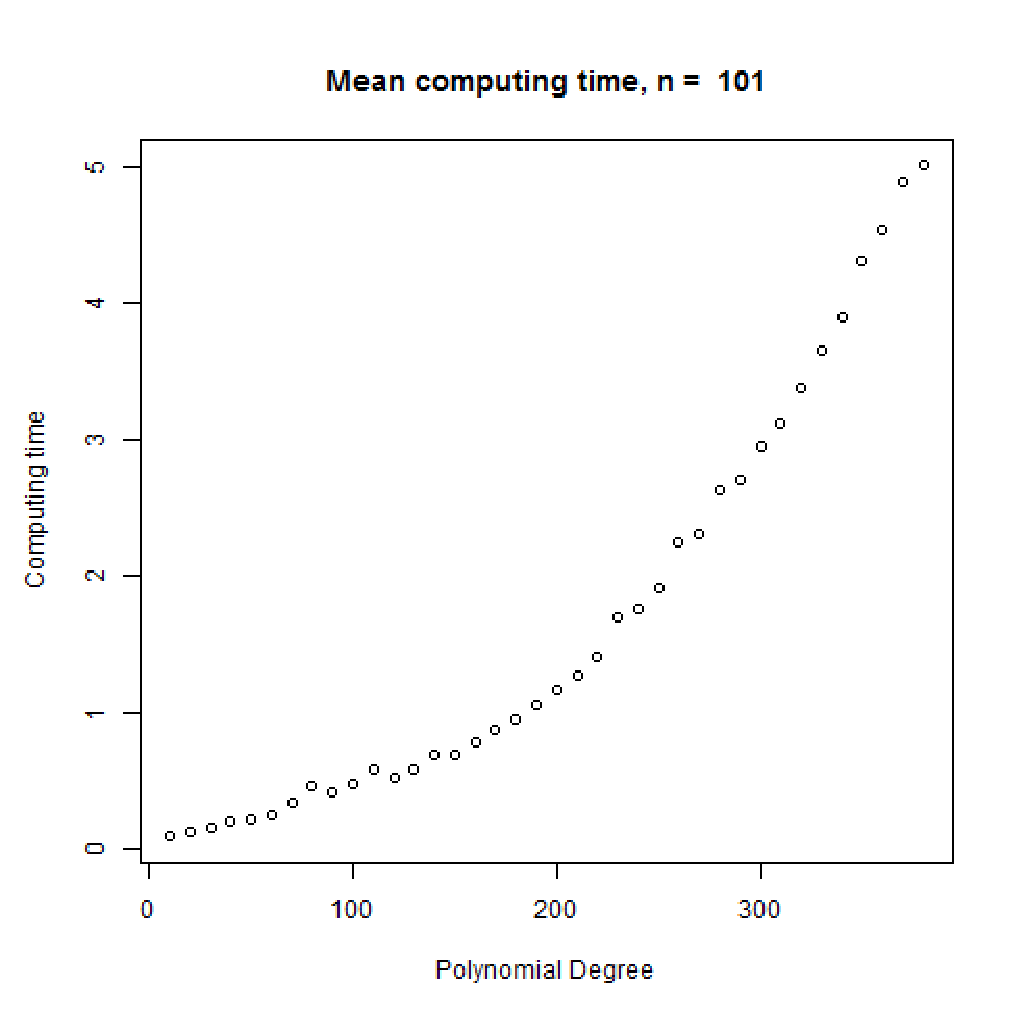
\includegraphics[width=3.50000in,height=3.50000in]{image17}
\caption{Tiempo de c\'omputo de simulaciones de la c\'opula de Bernstein en funci\'on del grado del polinomio.}
	\label{f:bernsPolyTime}
\end{figure}

Adem\'as, se detect\'o casi nula dependencia de las simulaciones con respecto al grado del polinomio:

\begin{figure}[H]
	\centering
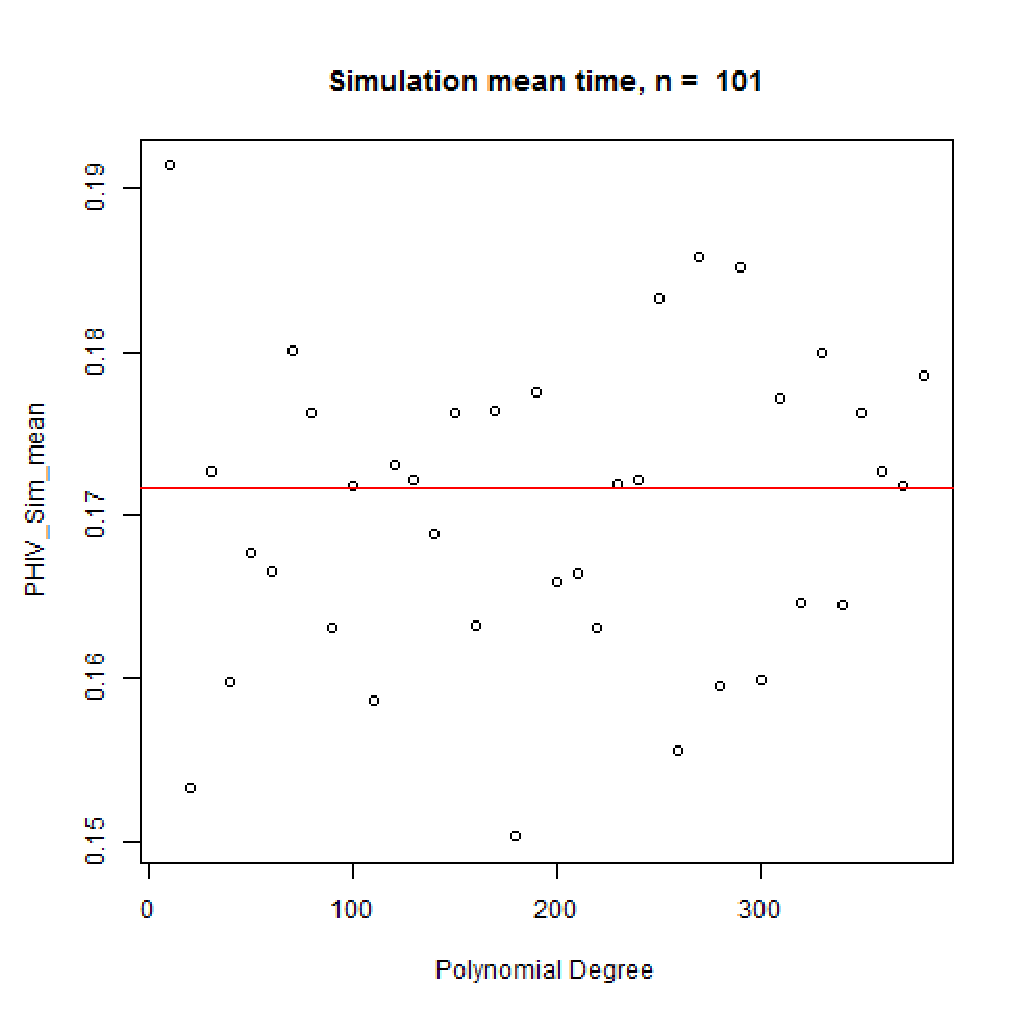
\includegraphics[width=3.00000in,height=3.00000in]{image18}
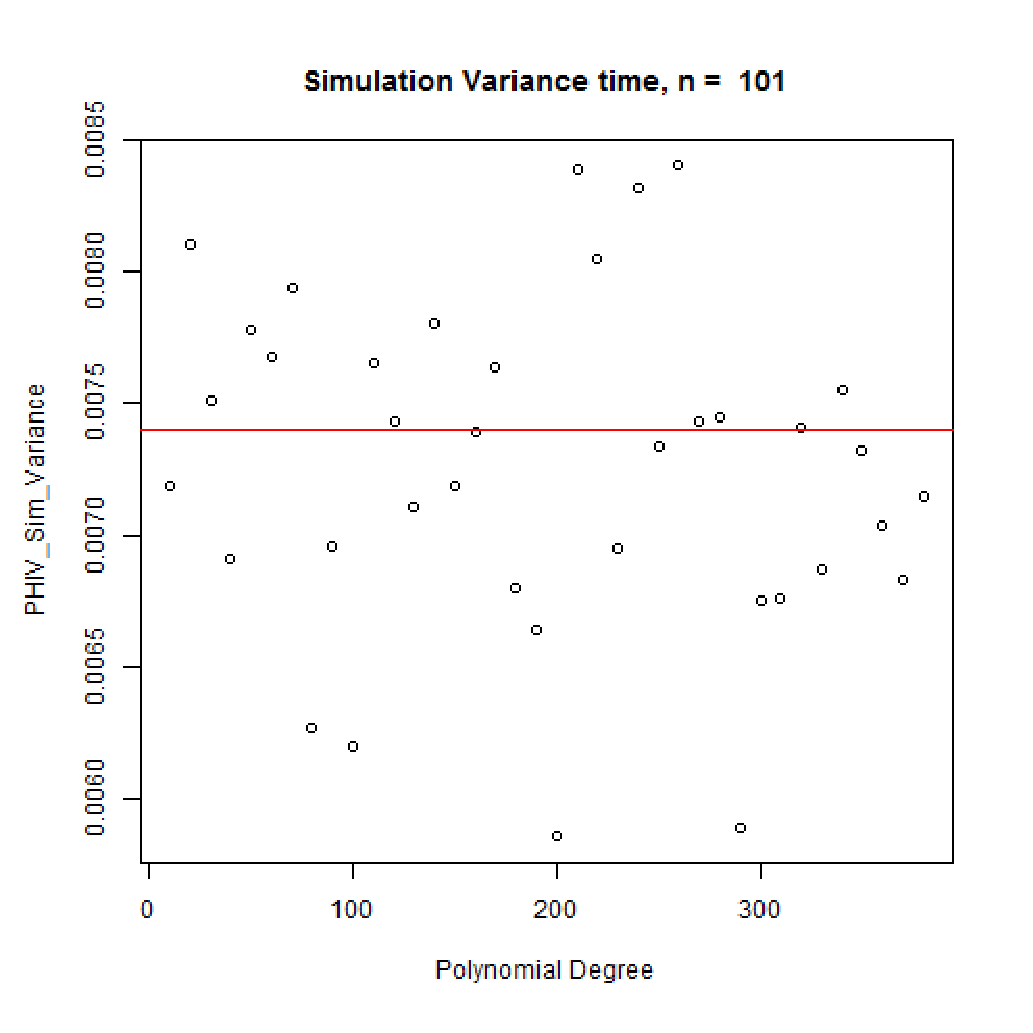
\includegraphics[width=3.00000in,height=3.00000in]{image19}
	\caption{Media (recuadro izquierdo) y varianza (recuadro derecho) en funci\'on del grado del polinomio de Bernstein de datos simulados.}
	\label{f:bernsPolyError}
\end{figure}

En todos los casos se utiliz\'o el mismo paquete desarrollado por los autores de este trabajo. La computadora utilizada es una laptop Lenovo ideapad z475, con 4 n\'ucleos y 4 Gb de memoria RAM.

